\subsection{Preprocesamiento De Los Datos} 
Con el objetivo de darle mayor estabilidad matematica a los datos y quitar algo del ruido que puedan tener, realizamos un preprocesamiento de los mismos. El mismo consistió en quitar los utliers dentro del set de datos y luego normalizarlos con media $0$ y varianza $1$.

\subsection{Implementacion Del algoritmo} 

El algoritmo que implementamos consistió en una red neuronal profunda con retropropagación del error. Este, descripto de manera informal consiste en introducir una instancia del problema, calcular la salida, compararla con la salida esperada y retropropagar el error, con el objetivo modificar las matrices de pesos y minimizar la diferencia. El sistema implementado se dice ser $online$ ya que los pesos de las matrices son ajutados luego de retropropagar el error de cada instancia en vez de hacerlo al final de la epoca.

A fin de tener una medida de como va "aprendiendo" la red neuronal, luego de presentarle a la red todas las instancias una vez, calculamos la norma de la diferencia entre las respuestas obtenidas y las esperadas. Consideraremos esta nuestra "norma del error" y la tomaremos como una metrica adecuada para saber cuan buenos resultados devuelve nuestra red.

%habria que poner pseudocodigo o algo mas lindo acá

%falta explicar un poco mejor las funciones de activacion que usamos, etc

Como optimización adicional se agrego un termino de momentum. La idea tras esto consiste en darle a cada peso de la matriz una "inercia" que le permita continuar avanzando en la direccion en la que avanzó en la iteración anterior. El objetivo consiste en disminuir las oscilaciones con cada pequeño cambio en la matriz.

\subsection{Experimentación sobre datos de Diagnostico de Cancer}

\subsubsection{Convergencia del algoritmo} 

%decir que usamos logistica porque es una clasificacion idem l.12

Para este problema utilizaremos una neurona en la ulima capa con función de activación logistica. Para ser consistentes con esto, las salidas esperadas adoptarán los valores $1$ si resulto ser cancer maligno, y $0$ si resulto ser benigno. La experimentación consistirá en buscar los parametros optimos que nos den la mayor tasa de aciertos para nuestro data set.

Como primera instancia comprobaremos que la red converge efectivamente a la solución esperada. Para eso tomamos un lerning rate de $0.01$, $7$ neuronas en la capa oculta y con $1300$ epocas graficamos la norma del error cada $1000$ iteraciones:

\begin{figure}[h!]
  \centering
    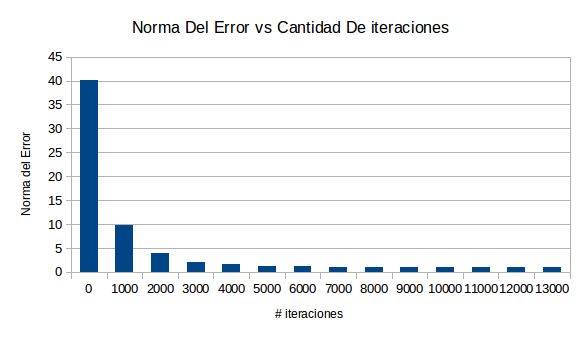
\includegraphics[scale=0.4]{ej1/convergencia.png}
\end{figure}

El grafico muestra que, efectivamente, nuestro algoritmo minimiza la diferencia entre las soluciones obtenidas y las deseadas, minimizando así tambien la norma del error.

En las secciones subsiguientes, realizaremos diferentes experimentaciones sobre los hiperparametros del algoritmo para intentar aproximar a la solcución ideal.

\subsubsection{Performance Vs Learning Rate} 

%Capaz va mas arriba?
Para evitar el sobreajuste las experimentaciones todas las experimentaciones desde este punto se realizarán con la siguente metodología. Se dividirá el set de datos de entrenamiento provisto por la catedra en dos sets de datos distintos. Uno se utilizará para entrenar la red, mientras que el otro se medirán que tan buenos fueron los resultados obtenidos. Con esto se espera reducir el overfittning que la red pueda generar y comprobar de manera mas acertada que tan buenos resultados dará la red sobre datos reales del problema.

Ademas, para visualizar los resultados mas claramente utilizaremos una matriz de confución, que nos permitirá dicernir entre falsos positivos (fp), falsos negativos(fn) y instancias clasificadas correctamente (tp y tn).

\reescribir 
%cantidad de neuronas!

En esta sección querremos experimentar es como se comporta el algoritmo al variar el learning rate. Para ello, dejamos constantes las cantidad de epocas de entrenamiento en $10000$ y variamos el learning desde $0.01$ hasta $0.2$ aumentando de a $0.01$

\begin{figure}[h!]
\centering
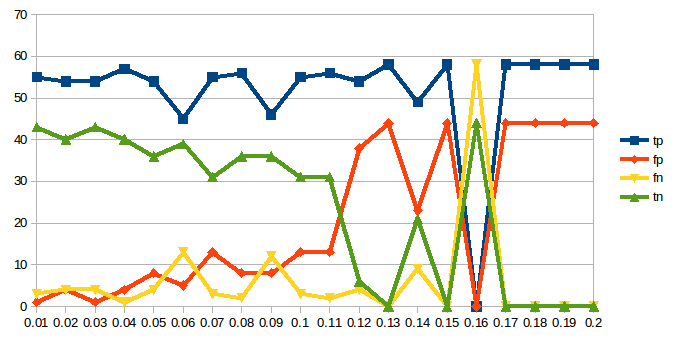
\includegraphics[scale=0.4]{ej1/test_learning_rate.png}
\end{figure}

El grafico muestra varios resultados interesantes. En el rango $[0.01,0.11]$ puede verse que la red arroja buenos resultados, obteniendo en general un $90\%$ de clasificaciones corrrectas. Pasado ese rango puede verse como los falsos positivos y los falsos negativos sufren un incremento muy significativo, llegando al final a casi un $50\%$ de clasificaiones incorrectas. Consideramos que para estos casos la red neuronal divergió, posiblemente debido a que multiplicar el gradiente por un valor muy grande lleva a "pasarnos" del minimo y por lo tanto reduciendo la precición del algoritmo. \completar

A partir de esta experimentación, para los siguientes experimentos decidimos tomar un learning rate igual a $0.02$. Concideramos que uno mayor puede producir que el altritmo diverga, mientras que uno mas pequeño hará que tarde demasiado en alcanzar la solución final.

\subsubsection{Performance Vs Cantidad De Neuronas} 

Otro experimento interesante para realizar es ver como cambia la calidad de los resultados dependiendo de la cantidad de neuronas en la red. Para probar esto mantenemos la cantidad de iteraciones y el learning rate fijos en $1000$ y $0.02$ respectivamente y variamos la cantidad de neuronas desde $1$ a $20$.

Los resultados obtenidos se grafican en el siguiente grafico:

\begin{figure}[h!]
\centering
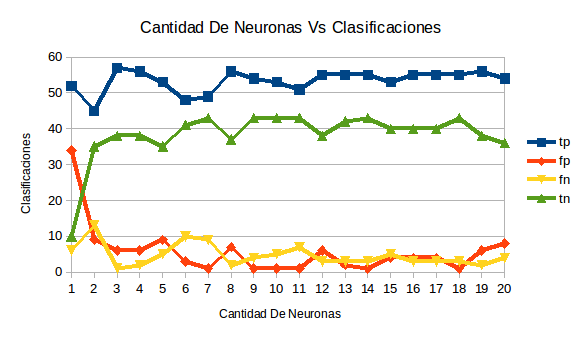
\includegraphics[scale=0.4]{ej1/test_neuronas.png}
\end{figure}

Como puede observarse, una cantidad de neuronas muy pequeña reduce considerablemente la calidad de los resultados. Esto puede deberse a \completar

En este caso decidimos utilizar una cantidad de neuronas igual a $3$. \porque

\subsubsection{Performance Vs Cantidad De iteraciónes} 

Como siguiete paso buscaremos analizar el comportamiento de la red para distintas cantidades de iteraciones, viendo si existe algun cambio significativo en este sentido. Para ello dejamos fijo el learning rate fijo en $0.01$ ya que consideramos que este nos da los resultados mas aceptables y variamos la cantidad de iteraciones.

\begin{figure}[h!]
  \centering
    \includegraphics[scale=0.4]{ej1/test_iter.png}
\end{figure}

Para una cantidad menor a $600$ iteraciones puede observarse que la red neuronal tiene una performance mala obteniendo un porcentaje de falsos negativos y falsos positivos cercano al $50\%$. Ya con $700$ iteraciones en adelante la performance del algoritmo mejora drasticamente, rondando el porcentaje de falsos negativos y falsos positivos al rededor de $10 \%$ y $20\%$. Para $2000$ y $2100$ iteraciones obtenemos un $7\%$  de falsos negativos.

Decidimos que la mejor cantidad de iteraciones en este caso será de $900$. El motivo de esta elección recide en lo antes expuesto, una cantidad menor produce que el algoritmo todavía no converga a la solción ideal, mietras que una cantidad mayor, si bien parece aumentar la precición de la solución, tambien podría deberse al overfitting de los datos.

\subsection{Eficiencia energética} 

%explicar modificacion?

Este problema presenta ciertas diferencias con respecto al anterior. En particular en este caso querremos hacer una regreción lineal sobre los datos. Por lo tanto, elegimos una función de activación lineal en la ultima capa. Ademas para cada conjunto de atributos se deverán volver dos resultados diferentes, por lo que la ultima capa tendrá dos neuronas de salida.

\subsubsection{Convergencia del algoritmo}

De igual manera que para el caso del cancer de mama, lo primero que querremos determinar es que el algoritmo comberge a la solución deseada. Por lo que nuevamente tomamos un lerning rate de $0.01$, $30$ neuronas en la capa oculta y con $100000$ epocas graficamos la norma del error cada $1000$ iteraciones:


\begin{figure}[h!]
  \centering
    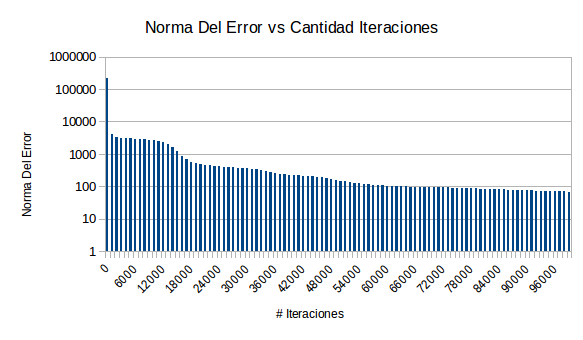
\includegraphics[scale=0.4]{ej2/convergencia.png}
\end{figure}

A simple vista se puede notar que en este caso el algritmo converge de manera mucho mas lenta (notar que el grafico se encuentra en escala logaritmica).

Podemos observar que el algoritmo efectivamente converge a la solución deseada. Nuestro siguiente objetivo será ajustar los parametros de manera adecuada para intentar que la solución devuelta por el algoritmo sea lo mas aproximada a la solución real.

\subsubsection{Performance Vs Learning Rate}

En esta sección esperamos determinar un learning rate adecuado para nuestro algoritmo. A priori pareciera que $0.01$ resulta muy bajo para este caso, resultando en una convergencia muy lenta. Para este experimento dejamos la cantidad de epocas fija en $10000$, la cantidad de neuronas de la capa oculta en $30$ y variamos el learning rate desde $0.01$ a $0.2$ con un step de $0.01$. Los resultados obtenidos fueron:

\begin{figure}[h!]
  \centering
    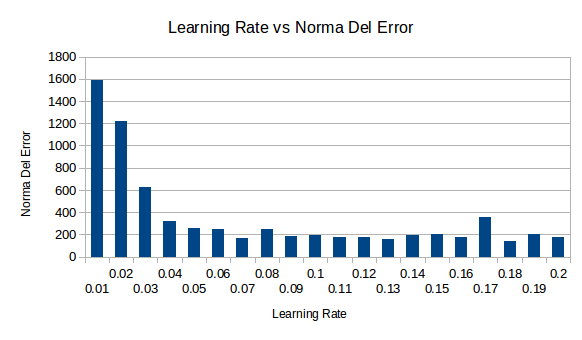
\includegraphics[scale=0.4]{ej2/test_learning_rate.png}
\end{figure}

Como puede verse, en este caso un learning rate mayor aumenta considerablemente la convergencia del algoritmo.

Por este motivo, elejimos como nuestro learning rate optimo el de $0.05$. Concideramos que un learning rate excesivo, si bien puede reducir la norma del error a niveles mayores, puede producir que el algoritmo no generalice las soluciones y simplemente memorice las instancias de entrenamiento.

\subsubsection{Cantidad De neuronas Vs Performance}

Al igual que en el caso del cancer, queremos ver como afecta la cantidad de neuronas a los resultados. Para ello nos basamos en el experimento anterior para obtener un learning rate que concideramos aceptable, dejamos la cantidad de iteraciones en $10000$ y variamos la cantidad de neuronas desde $1$ a $20$.

\begin{figure}[h!]
  \centering
    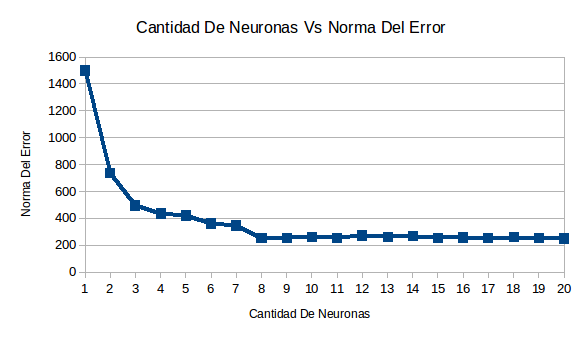
\includegraphics[scale=0.4]{ej2/test_neuronas.png}
\end{figure}

En el grafico puede observarse que para una cantidad muy pequeña de neuronas, los resultados resultan mucho peores. Aumentando la cantidad de neuronas a $3$ ya la norma del error mejora sustancialmente, mientras que para una cantidad mayor de neuronas el algoritmo parece alcanzar una meceta.

Por este motivo concideramos que para este caso la cantidad optima de neuronas es $8$.

%hablar sobre el overfitting si usamos parametros mayores o algo asi.

\subsubsection{Epocas Vs Performance}

Como experimento final para esta sección buscaremos encontrar cual es la cantidad optima de iteraciones para este algoritmo. Para ello utilizaremos los parametros que concideramos mejores en la experimentación anterior (cantidad de neuronas = 8 y learning rate = 0.02) y variamos la cantidad de epocas desde $2000$ hasta $21000$:

\begin{figure}[h!]
  \centering
    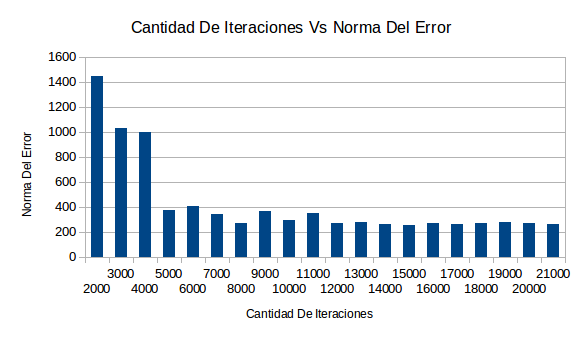
\includegraphics[scale=0.4]{ej2/test_iteraciones.png}
\end{figure}

Para $2000$ a $4000$ epocas, es correcto asumir que el algoritmo todavía no había convergido a una solución, encontrandose la norma del error en el orden de los $1000$. Desde las $5000$ iteraciones en adelante puede verse que el error cae repentinamente y se estabiliza en aproximadamente $200$.  

Por este motivo concideramos tomar para este caso una cantidad de epocas igual a $7000$.

%TODO: concluciones de cada apartado
